% Chapter Template

\chapter{Approach} % Main chapter title

\label{Chapter4} % Change X to a consecutive number; for referencing this chapter elsewhere, use \ref{ChapterX}

In this section, I present the design of my replacement for the Project EPIC infrastructure. The primary features of this infrastructure are:

\begin{itemize}
	\item Event management (creation/deletion/modification of events with specific keywords)
	\item Real-time collection of streaming Twitter data
	\item Real-time classification of incoming tweets (assigning tweets to active events)
	\item Data Analysis (performing queries on collected tweets using batch processing)
\end{itemize}

My goal is to recreate these features with less code and which is easier to deploy and update and is more flexible, scalable, and reliable than the existing infrastructure.

As mentioned above, my design will rely on a choreography-based microservices approach that is deployed on a cloud-based infrastructure making use of Docker and Kubernetes. My microservices will rely on Kafka to pass messages to one another via message queues (topics) that are created in response to requests to collect on crisis events.

One goal I have in my design is to make as many of my system components to be stateless. That is, these components will be designed to receive an incoming message from a Kafka queue that contains all the state they need to perform their operation. They will, in turn, generate messages that contain all the state that is needed for downstream components to process them. This design approach will pay dividends as it will allow the underlying container orchestration system to easily replace services that have crashed and to instantiate multiple copies of a particular service when there is a surge in demand for its services.

Not all of my components will be microservices. I will rely on Cassandra to persist the tweets that are collected; the reasons for using Cassandra have already been well documented in Project EPIC’s prior work \parencite{icse11,oopsla12,hiccs15}. Furthermore, I will be making use of Apache Spark to perform data analytics in my prototype and will provide a web-based \textit{notebook user interface} for the analysts to easily submit their queries and view the results. Examples of tools that provide notebook user interfaces for data analysis are Zeppelin and Project Jupyter.\footnote{\href{https://zeppelin.apache.org/}{https://zeppelin.apache.org/} and \href{http://jupyter.org/}{http://jupyter.org/}} These platforms integrate directly with Apache Spark and provide advanced features for viewing the results of Spark queries as tables and charts. The use of Apache Spark in my infrastructure was driven by the fact that it comes with a specialized \textit{Cassandra Connector} that allows it to perform queries on a cluster of Cassandra nodes efficiently. For instance, the Cassandra connector is smart enough to ``take the query to the data'' and perform a particular query distributed on the data stored in each Cassandra node rather than requiring data to be transferred between nodes before the query is performed. This feature is known as preserving \textit{data locality} and allows Apache Spark to perform queries on Cassandra in near real-time.

\section{Custom Components}

The specific components that I will be developing for my infrastructure are:

\begin{itemize}
	\item \textbf{Event Manager:} A web-based system that presents a user interface for managing data collection events. Each event has a name and a set of associated keywords. For instance, if a hurricane were to threaten the Eastern Seaboard of the United States, an event would be created using the hurricane’s name and the year it occurred. For example, ``2012 Hurricane Sandy.'' The list of keywords then specify items of interest related to that event; these words are typically place names (\texttt{new york city}), behavior-related terms (\texttt{evacuate}, \texttt{charging devices}, etc.) or event-specific terms (\texttt{flooding}, \texttt{smoke}, etc.). Submitting these terms to the Streaming API represents a request to collect every new tweet that contains one or more of these terms.

  Each time there is a change made to the current set of events, the Event Manager submits a message with all of the current events and keywords to a Kafka queue to report the change. The Event Manager  makes use of its own local database (SQLite) to ensure that its state is saved in the event of a crash.

	\item \textbf{Infrastructure Controller:} The infrastructure controller is responsible for issuing commands to Kubernetes to ensure that all instances of the microservices needed to collect the current set of events are up and running. It receives the messages generated by the Event Manager and updates the Twitter Tracker and Twitter Normalizers (both discussed next) to match the new state.

	\item \textbf{Twitter Tracker:} The Twitter tracker is a microservice that connects to the Twitter Streaming API, submits a set of keywords provided by the Infrastructure Controller, and then places each tweet that it receives in a Kafka message queue. If a change occurs, no tweet is missed as a new instance of the Twitter tracker is created and is receiving tweets before the old instance is taken down. All configuration for the Twitter tracker is handled via environment variables set by the container-orchestration system, making this microservice stateless.

	\item \textbf{Twitter Normalizer:} A Twitter normalizer is a microservice that gets assigned the keywords associated with a single event and is plugged into the Kafka queue that receives tweets from the Twitter Tracker. (This particular queue is configured such that all subscribers see all messages; in this case, each message contains a single tweet that was received from the Twitter Streaming API.) When a Twitter normalizer finds a tweet that contains one of its keyword, it normalizes that tweet to match the schema shown in Listing \ref{lst:cql} and stores the tweet in Cassandra.

  Note: since more than one event can specify the same keyword (for instance two hurricanes active at the same time may both contain \texttt{hurricane} as one of their keywords), a tweet may be stored multiple times by my prototype. Since most queries are focused on a particular event, this duplication is not an issue. However, if a query is specified across multiple events, then the onus is on the analyst to remove duplicate copies of a tweet before metrics are calculated.

  One Twitter normalizer is created for each event specified by the Event Manager. Of course, the Infrastructure Controller has the option of instantiating multiple instances of a Twitter normalizer if, for instance, it has determined that an event has been assigned a lot of high-frequency keywords but that particular functionality has not yet been implemented in my prototype.
\end{itemize}

Given these descriptions, the software architecture of my prototype is shown in Figure \ref{fig:SysArch}. In the next section, I will present more information about how my prototype is actually implemented.

\begin{figure}
\centering
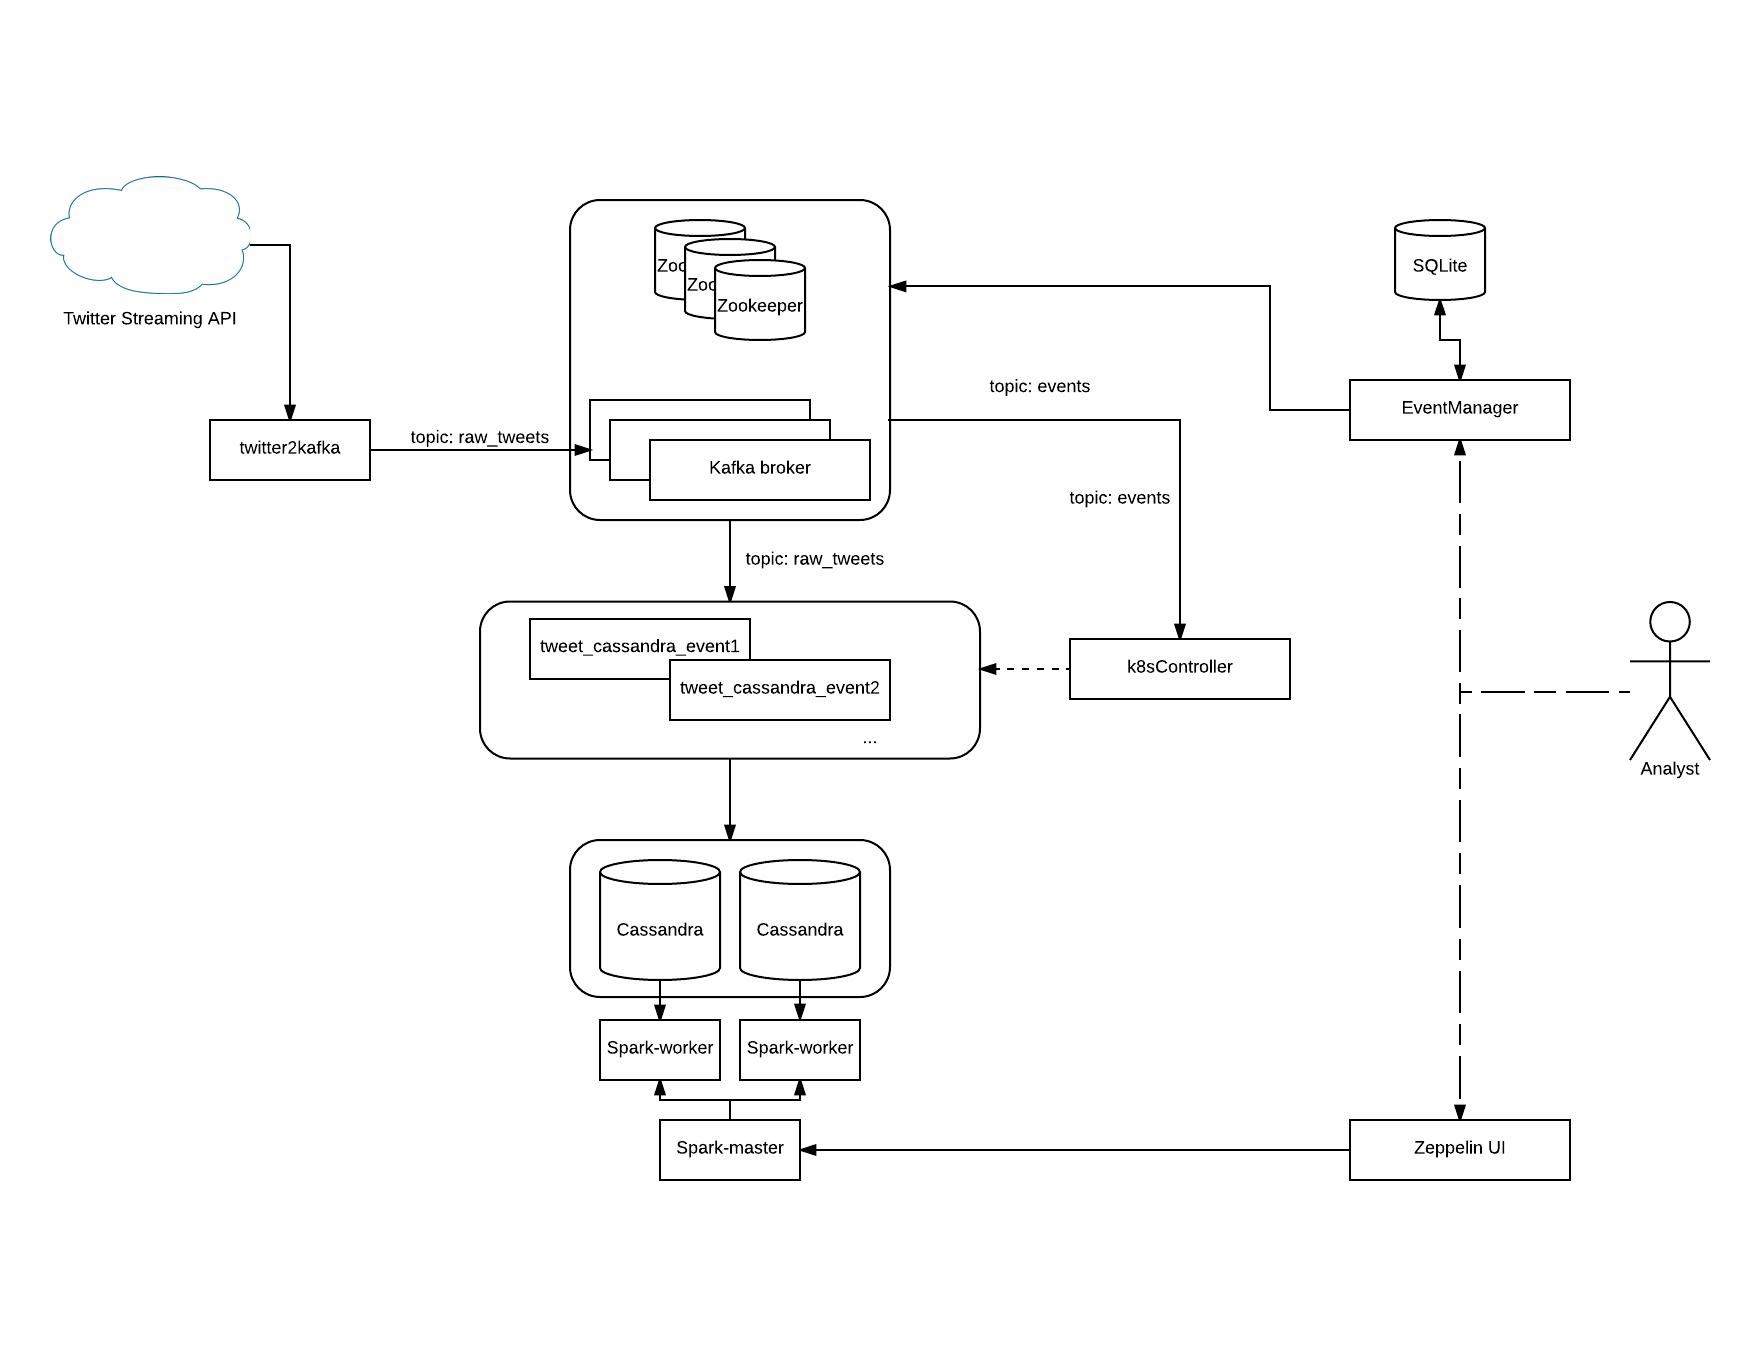
\includegraphics[width=\textwidth]{Figures/SysArch}
\decoRule
\caption[System architecture]{Proposed system architecture}
\label{fig:SysArch}
\end{figure}
